\section{Component Diagram}

Rispetto alla precedente iterazione, l’architettura del sistema è stata estesa mantenendo invariata la struttura a più livelli già adottata. In questo modo è stata conservata la separazione tra interfaccia utente, logica applicativa e gestione dei dati, introducendo però nuove funzionalità lato front-end e ampliando i componenti esistenti.

\begin{figure}[H]
    \centering
    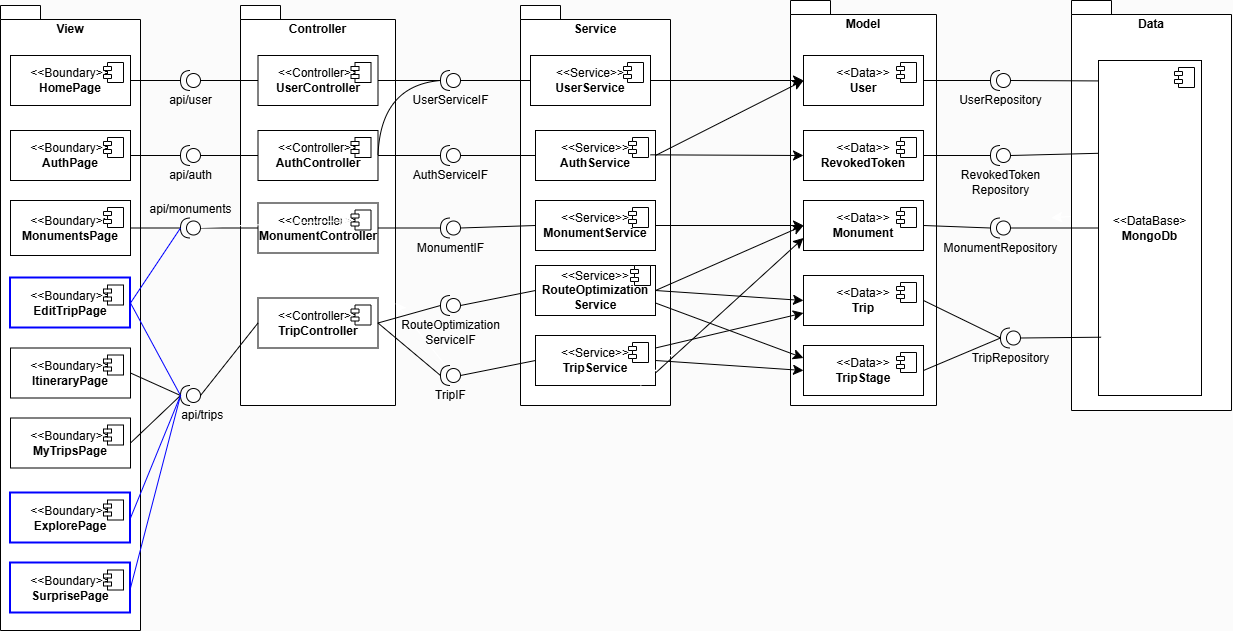
\includegraphics[width=\linewidth]{Iterazione2/Diagrammi/ComponentDiagramIt2.png}
    \caption{Diagramma dei componenti}
    \label{fig:ComponentDiagramIterazione2}
\end{figure}

In questa iterazione sono state aggiunte tre nuove pagine nel livello \textit{View}, ovvero \textit{ExplorePage}, \textit{SurprisePage} ed \textit{EditTripPage}. Gli altri livelli non introducono nuove classi, ma sono stati ampliati nelle funzionalità interne per supportare i nuovi casi d’uso e le nuove interazioni dell’applicazione.

Il diagramma mostra quindi un’evoluzione coerente dell’architettura: le nuove pagine del front-end sfruttano i controller esistenti, che delegano ai service aggiornati, i quali operano sulle entità del \textit{Model} e accedono ai dati attraverso il livello \textit{Data}. 